\PassOptionsToPackage{utf8}{inputenc}
\documentclass{bioinfo}

\copyrightyear{2020} \pubyear{2020}

\access{Advance Access Publication Date: day month 2020}
\appnotes{Application Note}

\usepackage{here}

\begin{document}
\firstpage{1}

\subtitle{Genetic and population analysis}

\title[MPCC]{MPCC: A high-performance matrix-based algorithm to compute Pearson correlation coefficients}
\author[Arends \textit{et~al}.]{
Danny Arends\,$^{\text{\sfb 1, $\dagger$}}$,
Mitch Horton\,$^{\text{\sfb 2, $\dagger$}}$,
Chad Burdyshaw\,$^{\text{\sfb 2, $\dagger$}}$,
Udit Gulati\,$^{\text{\sfb 3}}$,
Christian Fischer\,$^{\text{\sfb 4}}$,
Robert W. Williams\,$^{\text{\sfb 4}}$,
Pjotr Prins\,$^{\text{\sfb 4}}$,
Glenn Brook\,$^{\text{\sfb 2, *}}$}
\address{$^{\text{\sf 1}}$Z{\"u}chtungsbiologie und molekulare
Genetik, Albrecht Daniel Thaer-Institut, Berlin, 10115, Germany \\
$^{\text{\sf 2}}$The Joint Institute for Computational Sciences,
University of Tennessee, Oak Ridge, TN 37830, USA\\
$^{\text{\sf 3}}$Computer Science Department, Indian Institute of
Information Technology, Una, Himachal Pradesh, India\\
$^{\text{\sf 4}}$Department of Genetics, Genomics and Informatics, University
of Tennessee Health Science Center, Memphis, TN 38163, USA.}

\corresp{$^\dagger$Contributed equally and should be considered
joined first authors, $^\ast$To whom correspondence should be
addressed.}

\history{Received on XXXXX; revised on XXXXX; accepted on XXXXX}

\editor{Associate Editor: XXXXXXX}

\abstract{ \textbf{Motivation:} With the rapidly growing amount of 
  data acquired by high-throughput sequencing technologies, 
  combined with a growing body of phenotype data from medical and 
  experimental biology, computing correlation coefficients is a 
  recurring bottleneck. This bottleneck is amplified in the 
  presence of missing data.\\
\textbf{Results:} Here we present a novel high performance, 
  robust, matrix-based PCC algorithm that greatly reduces 
  the bottleneck associated with the PCC calculation, with any 
  amount of missing data. Our method is a reformulation of the
  standard Pearson correlation coeffient algorithm where
  the lion's share of the computation is handled by fast
  matrix-matrix products and element-wise matrix operations. 
  On a single Intel Xeon Gold 6148 $@$ $2.4$ GHz (Skylake) CPU our 
  algorithm achieves 4.3 TFlop/s in single  precision (i.e., 
  $77\%$ of the theoretical peak). We show how MPCC outperforms 
  the existing implementation in R by around $200$-fold. \\
\textbf{Availability:} Our source code is available as a C
  library for R published under a dual licence, the free and open
  source software GPL-v3 licence as well as the 3-Clause BSD License.
  Source code is available at: \href{https://github.com/UTennessee-JICS/MPCC}{https://github.com/UTennessee-JICS/MPCC}\\
\textbf{Contact:} \href{glenn-brook@tennessee.edu}{glenn-brook@tennessee.edu}\\
\textbf{Supplementary
  information:} Supplementary data are available
  at \textit{Bioinformatics} online.}

\maketitle


\section{Introduction}

The use of Pearson correlation coefficients (PCC) is ubiquitous across all 
fields of biology ranging from agriculture to zoology. Large-scale 
computation of correlations are found in many areas of biology and 
bioinformatics.  For example, genotype-genotype correlations are 
used to construct haplotypes, build genetic maps, and order markers 
within the genome. Pearson correlations are also used in 
co-expression analysis \citep{Tesson:2010}, (genome wide) 
association analysis \citep{Cichonska:2016}, reconstruction of genetic
networks \citep{Fukushima:2013}, weighted correlation network analysis
(WGCNA) \citep{Horvath:2008} and correlated trait locus (CTL)
mapping \citep{Arends2016a}.

\enlargethispage{12pt}

The work presented here is motivated by GeneNetwork, a service for
web-based genetics \citep{Sloan2016} which routinely performs PCC 
calculations to find relationships between and among genotypes and 
phenotypes. These calculations are a bottleneck when faced with 
moderate to large problem sizes.

The BXD family is a panel of 150 recombinant inbred mouse lines
derived from parents C57BL/6J and DBA/2J \citep{Ashbrook:2019}. The
BXD data collection in GeneNetwork consists of high-density genotypes
with 7,000 classical phenotypes and over 120 independent data sets containing
between 20,000 to 1.2 million gene expression phenotypes. Consider 
the problem size when PCC are computed within or between sets 
of gene expression phenotypes. 

Statistics are often computed in the R language for statistical computing 
\citep{R:2005}. R's default $cor()$ implementation of PCC is written in C, 
and while relatively performant on complete data, it is especially slow 
when handling missing data. The default option to remove individuals with 
missing phenotype or genotype data does is not suitable for most biological 
data sets. In GeneNetwork, for example, most data set use different subsets 
of the available 150 BXD lines. A PCC computation based on removing rows with 
missing phenotypes would simply end up being empty. 

With MPCC we implemented a novel matrix based approach for PCC 
computation, that is a drop-in replacement for R's default $cor()$ 
function and can handle missing data without loss of performance.
\vspace*{-4mm}

\begin{figure}[H]
\centering
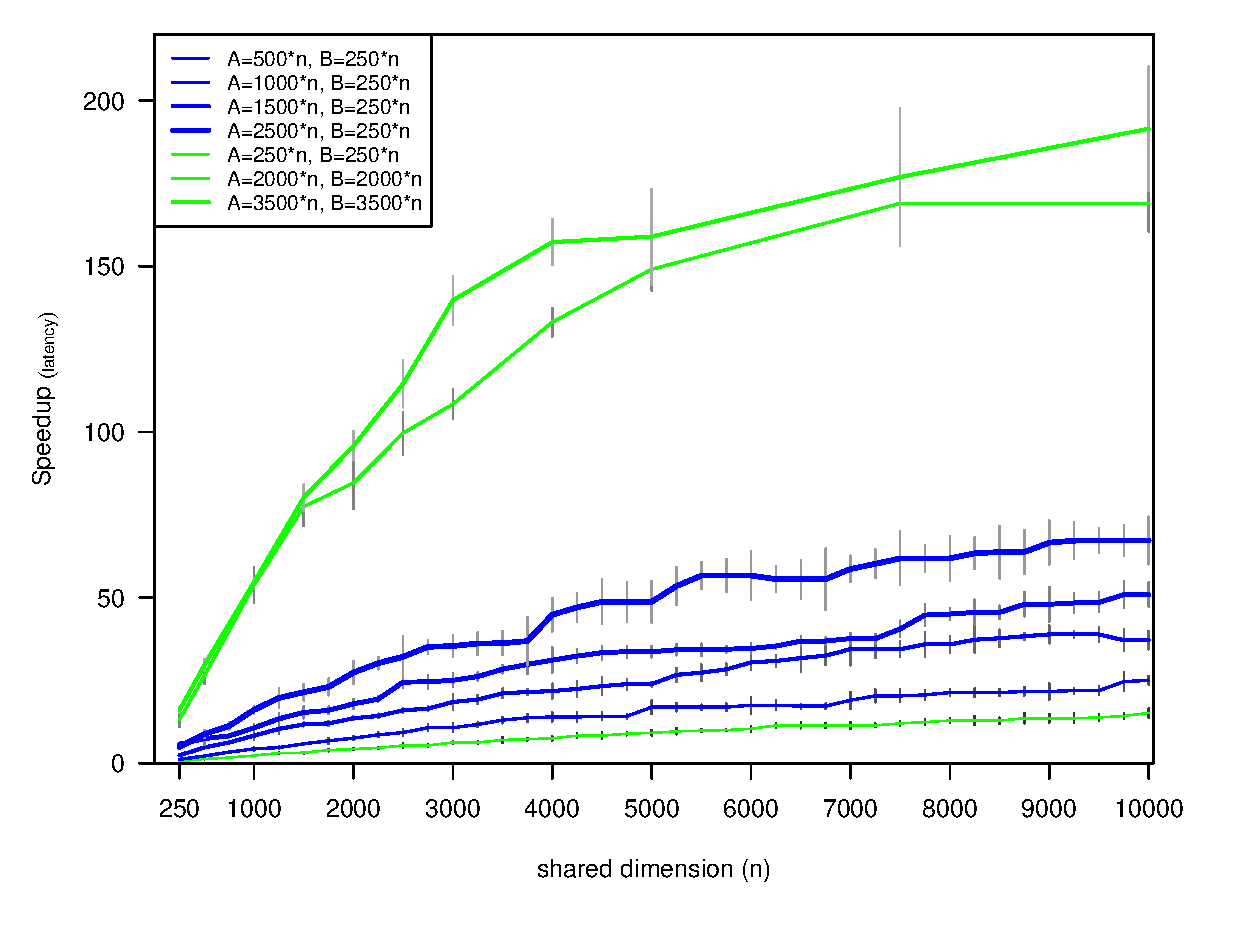
\includegraphics[width=\linewidth]{img/figure02big.eps}
  \vspace{-8mm}
  \caption{ \small Speed comparison of MPCC versus the native R $cor()$
  function shows increased performance with increased matrix
  sizes. Square matrices (blue) run faster than the non-square
  matrices (red).  The effect of handling missing data (0 to 50\%) is
  visualized with error bars - i.e. these show that missing data
  handled by MPCC bit-masking has limited effect on performance.
  Multi-threaded performance for a 3500x3500 matrix shows a potential
   \textasciitilde{}$200$-fold speedup compared to the default $cor()$ function.  All
  timings were performed on a system with 28 cores (56 hyper-threads)
  Intel(R) Xeon(R) CPU E5-2680 v4 @ 2.40GHz.  } \label{fig:fig1}
\end{figure}

\vspace*{-12mm}

\section{Approach}

We started work on optimizing the speed at which correlations are computed 
by writing a version that is algorithmically identical to the R $cor()$ function
(Supplement 1 and 2). To this version OpenMP multi-threading support was added. 
This provided a limited speedup, typically in the order of
3.5$\times$ compared to the single core version. 

In the next iteration, we wrote MPCC, an implementation of PCC that can 
leverage the advantages offered by any math library that is optimized 
for matrix-based operations, such as Intel’s Math Kernel Library (MKL), 
IBM’s Engineering and Scientific Subroutine Library (ESSL), the AMD 
Core Math Library (ACML), and Nvidia’s CUBLAS. This approach sped up 
computations up to $200\times$ on a 28-core machine (Fig. \ref{fig:fig1}). 
MPCC reformulates the original algorithm into a series of matrix-matrix 
products and element-wise matrix operations (Supplement 3 - 'The Matrix Version'). 

MPCC handles missing data by using a novel bit-masking approach that
leverages existing matrix-matrix multiplication implementations from,
for example, OpenBLAS (Supplement 4 - 'Missing Data Bit-masking').

To benchmark MPCC on a real-world problem pairwise correlation between 
genotypes of the BXD family were computed. Genotype data in the BXD 
family is complete with only a few heterozygous or 'missing' loci 
remaining, i.e., it benchmarks MPCC versus $cor()$ when only a small amount
of data is missing (Supplemental Fig. 1). Furthermore, speed improvement of MPCC
versus R's $cor()$ were computed using randomly generated phenotype matrices. 
We step-wise increased the size of the matrices as well as the amount of 
missing data. Even on a single core MPCC showed a \textasciitilde{}$5$-fold 
speedup compared to the $cor()$ function provided in R. With multi-threading 
MPCC gains with every core added, up to \textasciitilde{}$200$-fold in our 
tests (Fig. \ref{fig:fig1}).

MPCC can be installed as an R package. MPCC is written in C$++$, and
provides a foreign function interface (FFI). MPCC can therefore be
called from any other computer language using FFI. The source
repository includes an FFI binding for the R programming language
which can act as an example for other programming languages.

%\vspace*{2mm}
\section{Discussion}

MPCC is a reimplementation of the original PCC algorithm using matrix-matrix 
multiplication and element-wise matrix operations. MPCC makes use of 
multi-threading and modern vector extensions of CPU hardware. The missing 
data bit-masking approach can handle missing data without loss of performance, 
and can be generalized to other algorithms which rely on matrix-matrix multiplication. 

MPCC as well as the missing data bit-masking approach were recently ported 
to run on a GPU. However, the GPU implementation has not yet been added to 
the R package distribution. The GPU implementation is available using the FFI, and 
will be made available from the R package in the near future.

With this work we not only introduce a faster routine that reduces
regularly occurring bottlenecks in large-scale correlation computations, but
also show that it can pay off to revisit 'obvious' implementations
of routines in common use today that were written over 20 years
ago. Computer hardware and architecture is still changing and
dedicated optimization work may benefit both interactivity for
end-users and large-scale computations on high-perfomance compute
clusters at the same time.

\section*{Funding}

We thank the support of XSEDE/NSF startup MCB190140, the UT Center for
Integrative and Translational Genomics, and funds from the UT-ORNL
Governor's Chair, NIGMS Systems Genetics and Precision Medicine
Project R01 GM123489, NIDA grant P30 DA044223, NIAAA U01 AA013499 and
U01 AA016662.\\
\textit{Conflict of Interest:} none declared.

\vspace*{-5mm}
\bibliographystyle{natbib}
\bibliography{main}

\end{document}
